%\exer{}
\setcounter{numques}{0}

\begin{wrapfigure}{r}{5cm}
%\caption{A wrapped figure going nicely inside the text.}\label{wrap-fig:1}
\centering
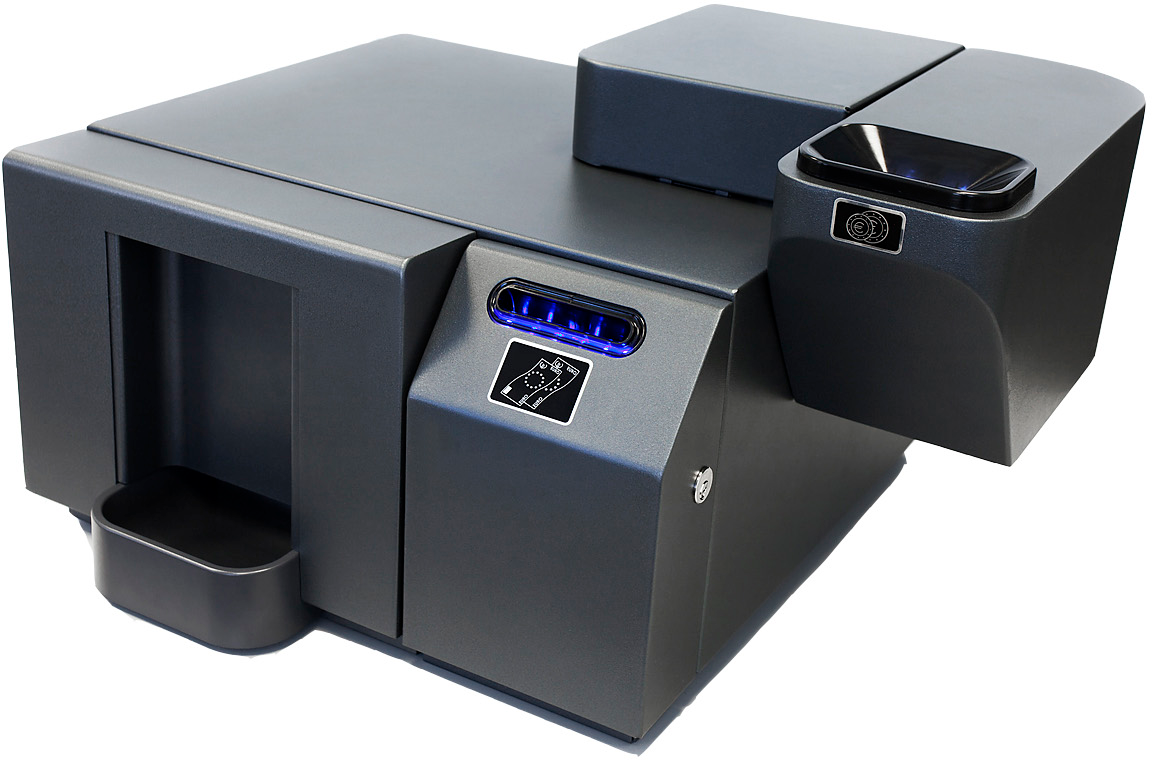
\includegraphics[width=4cm]{sharp.png}
\end{wrapfigure} 

La société Sharp commercialise des caisses automatiques utilisées par exemple dans des boulangeries. Le client glisse directement les billets ou les pièces dans la machine qui se charge de rendre automatiquement la monnaie. 
\begin{obj}
Afin de satisfaire les clients, on cherche à déterminer un algorithme qui va permettre de rendre le moins de monnaie possible. 
\end{obj}

La machine dispose de billets de 20\euro{}, 10\euro{} et 5\euro{} ainsi que des pièces de 2\euro{}, 1\euro{}, 50, 20, 10, 5, 2 et 1 centimes. 

\vspace{.5cm}

On se propose donc de concevoir un algorithme qui demande à l'utilisateur du programme la somme totale à payer ainsi que le montant donné par l'acheteur. L'algorithme doit alors déterminer quels sont les billets et les pièces à rendre par le vendeur. 

\textbf{Pour ne pas faire d'erreurs d'approximation, tous les calculs seront faits en centimes.}

Le contenu de la caisse automatique et le contenu du porte-monnaie du client seront modélisés par un tableau ayant la forme suivante : 
\begin{lstlisting}
caisse = [[2000,5],[1000,5],[500,5],[200,5],[100,5],[50,5],[20,5],[10,5],[5,5],[2,5],[1,5]]
\end{lstlisting}
Cela signifie que la caisse contient 5 billets de 20\euro{}, 5 billets de 10\euro{}... 
%client = {"2000":10,"1000":0,"500":0,"200":0,"100":0,"50":0,"20:":0,"10":10,"5":10,"2":0,"1":0}

%\question{}Créer une liste {valeurs} contenant toutes les valeurs des billets ou pièces.

%\question{}
%Pour un montant d'achat donné et pour une somme donnée par le client, proposer un algorithme en pseudo code permettant de rendre le minimum de monnaie au client. Cet algorithme devra détailler la somme à rendre (nombre de pièces et nombre de billets).


\textbf{Dans la prochaine question, on fait l'hypothèse que la caisse contient suffisamment de billets et de pièces de chaque valeur.}

\question{Ecrire une fonction \texttt{rendre\_monnaie(caisse:list, cout:float, somme\_client:float)-> list} prenant en arguments deux flottants \texttt{cout} et \texttt{somme\_client} représentant le coût d'un produit et la somme donnée par le client en \euro{} ainsi que le contenu de la caisse. Cette fonction renvoie la liste des billets à rendre par le client.}

Ainsi, l'instruction \texttt{rendre\_monnaie(caisse, 16, 20)} renvoie la liste \texttt{[200, 200]}. 

\texttt{rendre\_monnaie(caisse,15.92,20)} renvoie \texttt{[200, 200, 5, 2, 1]}


\question{Ecrire une fonction \texttt{rendre\_monnaie\_v2(caisse:list, cout:float, somme\_client:float)-> list} ayant le même objectif que la précédente. Cette fonction devra de plus mettre à jour la caisse. Elle devra prendre en compte que la caisse peut manquer de billets. Elle renverra une liste vide s'il n'est pas possible de rendre la monnaie.}

Pour l'instruction \texttt{rendre\_monnaie\_v2(caisse, 15.99, 200)}, la liste renvoyées est la suivante :
\texttt{[2000, 2000, 2000, 2000, 2000, 1000, 1000, 1000, 1000, 1000, 500, 500, 500, 500, 500, 200, 200, 200, 200, 100, 1]}. Le contenu de la caisse est alors : \texttt{[[2000, 0], [1000, 0], [500, 0], [200, 1], [100, 4], [50, 5], [20, 5], [10, 5], [5, 5], [2, 5], [1, 4]]}.

L'instruction \texttt{rendre\_monnaie\_v2(caisse, 15.99, 200)} renvoie \texttt{[]}.

On suppose que la caisse est maintenant la suivante. 
\begin{lstlisting}
caisse = [[5000,10],[2000,10],[1000,10],[800,10],[100,10]]
\end{lstlisting}

Le client achète un article de 34\euro{} avec un billet de 50\euro{}.

\question{Que retourne la fonction \texttt{rendre\_monnaie} ? Est-ce le rendu optimal ? Conclure << qualitativement >>.}

Pour l'instruction \texttt{rendre\_monnaie\_v2(caisse, 34, 50)}, l'algorithme renverra \texttt{[1000, 100, 100, 100, 100, 100, 100]}.

